\chapter{Réalisation de la toolbox}

\section{Introduction}

Dans ce chapitre, nous introduisons l'implémentation de notre projet. D'abord, nous 
décrirons les différents outils utilisés pour la réalisation de la toolbox. Ensuite,
nous possèderons à démontrer notre toolbox de Dempster-Shafer en détaillant ses
fonctionnalitées. Enfin, nous présentons la grande toolbox qui regroupe plusieurs
logiciels reliée aux théories de l'incertain.

\section{Les languages de programmations et les bibliothèques utilisés}

Nous avons programmé l'interface de la toolbox de Dempster-Shafer en \textbf{Python 3}
en utilisant la bibliothèque \textbf{PyQt4}. Nous avons également réalisé la grande
interface avec \textbf{Java Swing}.

\section{La toolbox de Dempster-Shafer}

Ce logiciel est constitué à partir de deux parties, le noyau et l'interface graphique.
Il peut fonctionner sur tout les systèmes d'exploitations majeurs comme \textbf{Windows},
\textbf{Mac~OS~X}, \textbf{GNU/Linux} et \textbf{BSD}.

Le noyau est responsable d'effectuer les calculs après la lecture d'un fichier XML
contenant les données nécessaires pour l'application de la théorie de Dempster-Shafer.
Les résultats seront écrits dans un autre fichier XML. L'utilisateur n'a pas besoin
de comprendre la structure de ces fichiers, il suffit juste d'utiliser l'interface
graphique.

L'interface graphique est composée d'une barre de menu et de trois parties, les états
du monde, les hypothèses, et les agents. La barre contient les fonctionnalités principales
pour enregister, ouvrir, réinitialiser le projet et fermer l'application dans le menu
\textbf{Fichier}. Dans le menu \textbf{Projet}, on trouve les actions liés à la manipulation
du projet courant. On peut y changer le titre et donner une description au projet. 

\begin{figure}[H]
\begin{subfigure}{0.49\textwidth}
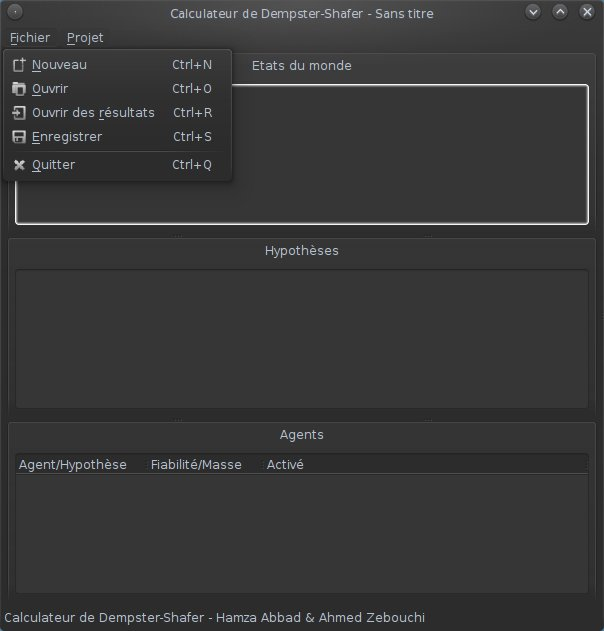
\includegraphics[width=\textwidth]{Inetrface_principale_menu_fichier}
\caption{Le menu \textbf{Fichier}}
\end{subfigure}
\hfill
\begin{subfigure}{0.49\textwidth}
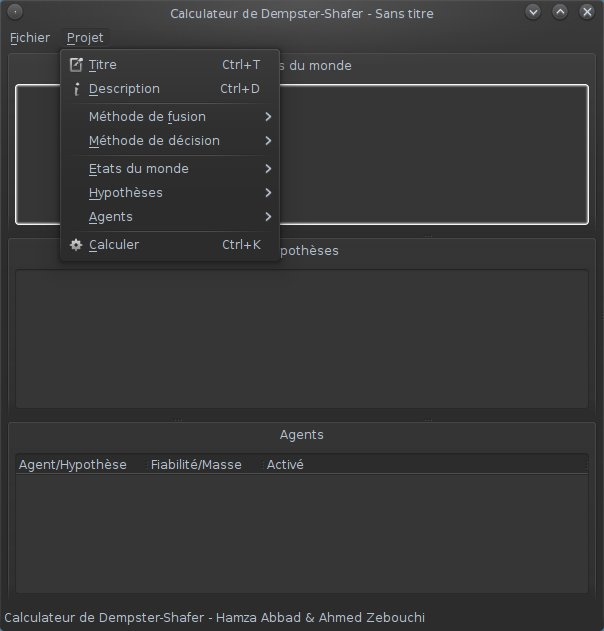
\includegraphics[width=\textwidth]{Inetrface_principale_menu_projet}
\caption{Le menu \textbf{Projet}}
\end{subfigure}
\caption{L'interface principale de la toolbox de Dempster-Shafer}
\end{figure}

Les états du monde, les hypothèses et les agents doivent s'ajouter dans cet ordre à partir
de ce menu ou par un clique droit dans leurs champs. \`A partir de ce menu, on peut choisir la
méthode de fusion et la méthode de décision.

On commence par ajouter tout les états du monde. Ensuite, à chaque fois on sélectionne certains
états et on établit une hypothèse à partir de ces états.

\begin{figure}[H]
\begin{subfigure}{0.49\textwidth}
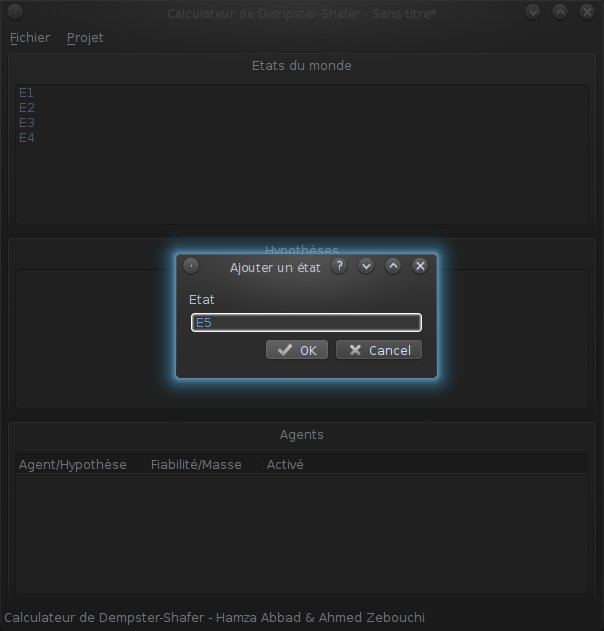
\includegraphics[width=\textwidth]{ajouter_etat}
\caption{Ajouter les états du monde}
\end{subfigure}
\hfill
\begin{subfigure}{0.49\textwidth}
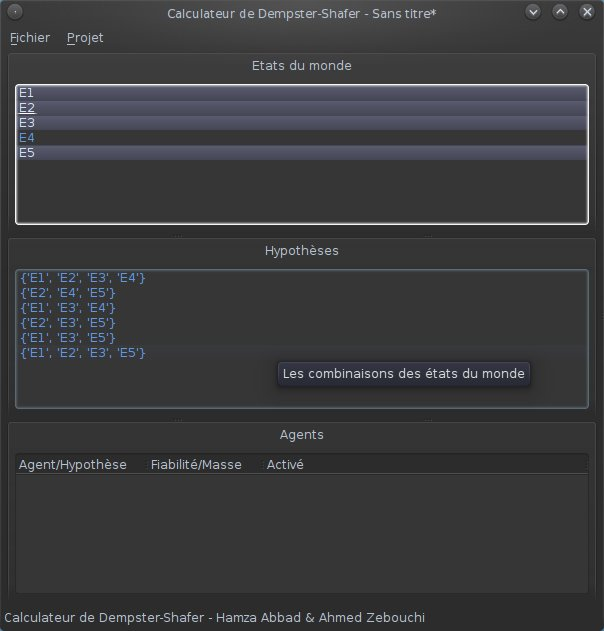
\includegraphics[width=\textwidth]{ajouter_hypothese}
\caption{Ajouter une hypothèse à partir des états}
\end{subfigure}
\caption{L'ajout des états du monde et les hypothèses}
\end{figure}

Par la suite, on doit procéder à ajouter les agents. Chaque agent doit avoir un nom, un niveau de
fiabilité et des hypothèses tels que à chaque hypothèse est affectée à une masse.

\begin{figure}[H]
\begin{subfigure}{0.49\textwidth}
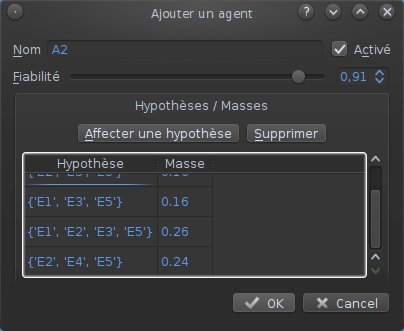
\includegraphics[width=\textwidth]{ajouter_agent}
\caption{Dialogue de l'ajout d'un agent}
\end{subfigure}
\hfill
\begin{subfigure}{0.49\textwidth}
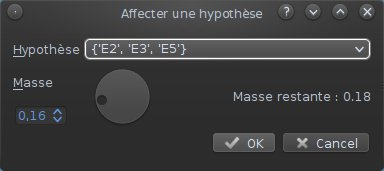
\includegraphics[width=\textwidth]{affecter_masse}
\caption{Dialogue de l'affectation d'une hypothèse}
\end{subfigure}
\caption{L'ajout d'un agent et l'affectation de ses hypothèses}
\end{figure}

Avant de passer au calcul, on doit enregistrer ces données dans un fichier. On doit choisir son nom
et son emplacement. Il aura par défaut l'extention \texttt{.dsti.xml}. Si on ignore cette étape le programme
demandera de la faire avant qu'on puisse continuer.

\begin{figure}[H]
\centering
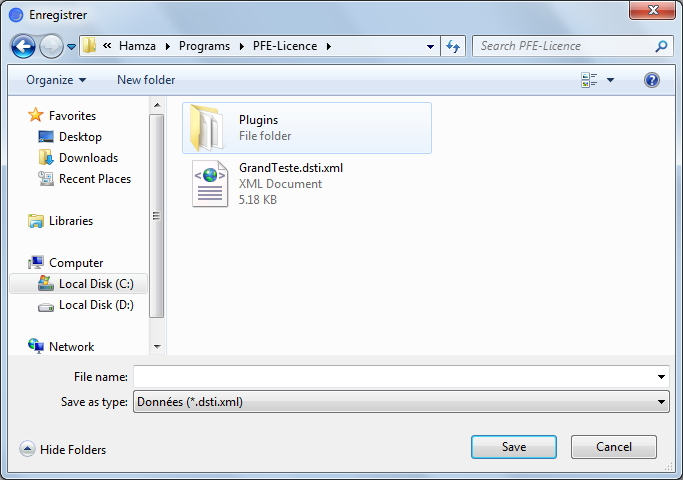
\includegraphics[width=0.8\textwidth]{Enregistrer}
\caption{Enregistrer les données}
\end{figure}

Enfin, on peut lancer le calcul. Cette étape risque de prendre un temps impotant si le nombre des états
du mondes et/ou des agents est assez grand. Pour cela, un dialogue d'attente est affiché pendant l'exécution
du noyau en arrière-plan. L'utilisateur peut annuler cette opération à tout moment.

Quand le calcul se termine, un dialogue contenant tout les résultats sera affiché. Les résultats sont obtenus
par la lecture du fichier généré par le noyau qui a le même chemin que le fichier sauvegardé sauf qu'il porte
l'extention \texttt{.dsto.xml}.

\begin{figure}[H]
\begin{subfigure}{0.39\textwidth}
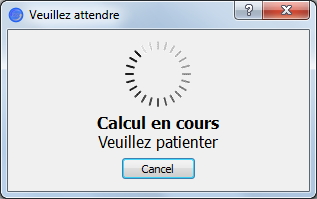
\includegraphics[width=\textwidth]{Dialogue_attente}
\caption{Dialogue d'attente}
\end{subfigure}
\hfill
\begin{subfigure}{0.59\textwidth}
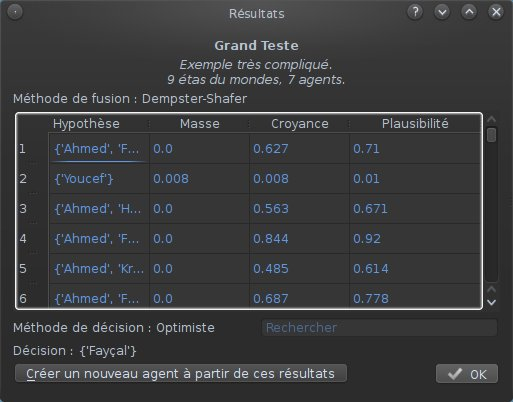
\includegraphics[width=\textwidth]{Dialogue_resultats}
\caption{Dialogue des résultats}
\end{subfigure}
\caption{Le calcul et l'affichage des résultats}
\end{figure}
